\section{Split-DASH System Architecture}
\label{sec:Split_DASH_architecture}
To solve above problem we propose Split-DASH architecture. In split-DASH architecture, we split the original DASH architecture into two parts, i) a dumb player or client and ii) a smart server side. The proposed architecture depicted in the Fig.~\ref{fig:playerDiagram_split}.
\begin{figure}[ht]
	\begin{center}
		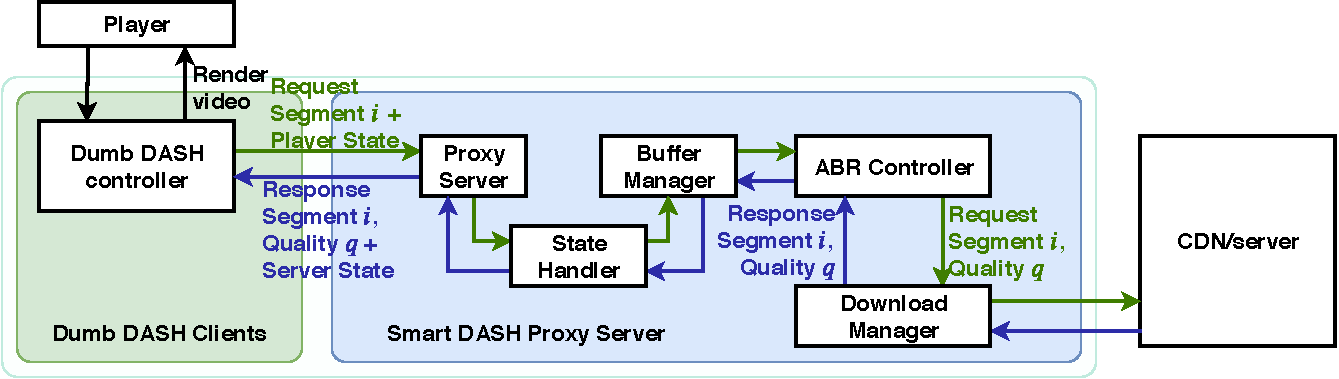
\includegraphics[width=0.9\linewidth]{img/playerDiagram_split}
	\end{center}
	\caption{\label{fig:playerDiagram_split} Modified DASH based streaming system to support ML-based ABR algorithm}
\end{figure}
Here we make the player dumb. It controls the playback; however, it does not take any decision. Instead, it depends on the decision provided by the smart counterpart in the server. The server provides the following decision: i) time to download a segment, and ii) quality of the segment. Before we explain the functionality of different modules in the server and client, we explain the transaction between the dumb-client and the smart server. 

\begin{figure}[h]
	\begin{center}
		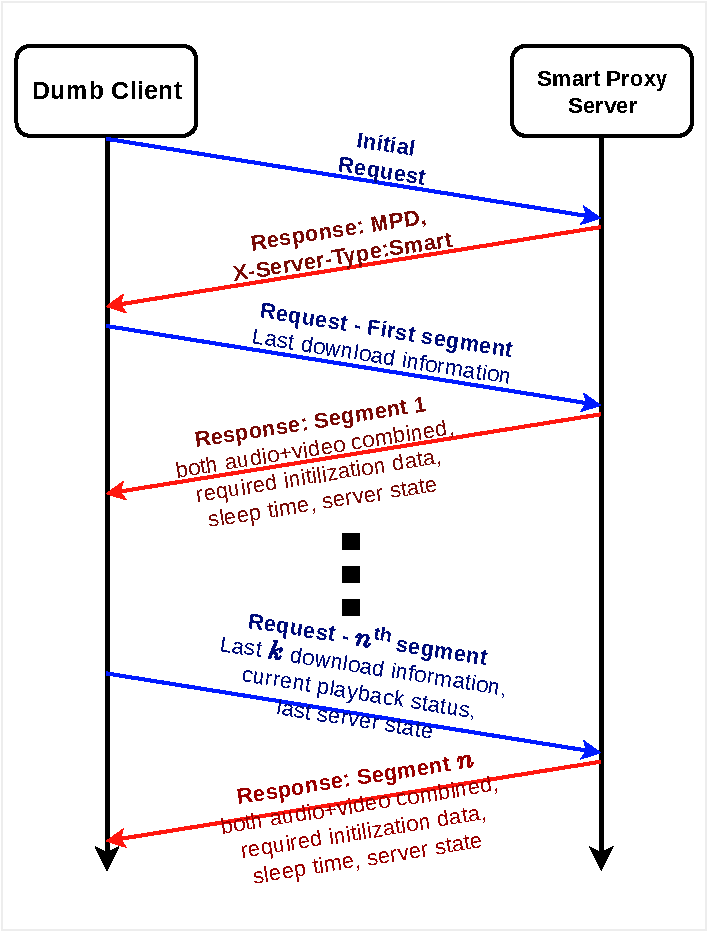
\includegraphics[width=0.5\linewidth]{img/splitDASHTransaction}
	\end{center}
	\caption{\label{fig:splitDASHTransaction} Modified DASH based streaming system to support ML based ABR algorithm}
\end{figure}

The Fig.~\ref{fig:splitDASHTransaction} depict the transaction between a smart proxy server and its dumb counterpart client. At first client request the Media Presentation Description (MPD) from the server. The smart proxy server returns an un-modified MPD for the video. However, it also adds a server identifier {\tt X-Server-Type: Smart}. This identifier indicates that the server is not a simple CDN server; instead, it is a smart proxy server. So, the dumb client prepares the HTML video element and request for the first video segment.

Here client does not mention the video/audio quality for the segment. Instead, the client encloses the download history with the request. When the server receives a request, it looks for the old server state in the request. If present, it expands the state; otherwise, it creates a new state. After that, it updates the state according to the current playback information and downloads the history provided in the request. Based on this information, the server calculates the best quality for both audio and video segments based on the pre-decided ABR algorithm. Once the quality is decided, it downloads the required segments of the calculated quality from the CDN/streaming (if not available in its cache) and sends the same back to the dumb player. It also calculates the time player should wait (\ie sleep time) before sending another request to the server. It multiplexes the sleep time and server state with the request. The contents of the server state are dependent on the ABR algorithm. Most of the deterministic ABR algorithm does not require to maintain any state. However, the ABR algorithm, like Pensieve, need to maintain state. In the case of the Pensieve ABR algorithm, the server state contains only the Pensieve state.
Here we send the server state to the client to make server stateless. The client does not read the server state. However, it stores the state in its memory and sends it to the server with the next request. As the server state contains all the information regarding the previous server state, the client can send the same request multiple times and with server responses with the same action for all of them. This very important as a response might get lost, and the client might need to resend the request to the server.

\noteam{need to add overhead with a table or plot}
